    Figure \ref{pipeline} shows our data pipeline. Data is imported from the NXT switchboard corpus \cite{calhoun2010nxt} into a graph database \cite{Webber:2012:PIN:2384716.2384777}.
   Figure \ref{datastructure} shows the data structure as it is represented inside the graph database. For each conversation, the conversation entities (words, dialog acts and turns) are represented as edges between time points, which are represented as vertices. The structure leads to a direct computation of the summary features using the graph query language.
\begin{figure}[ht!]
 \centering
 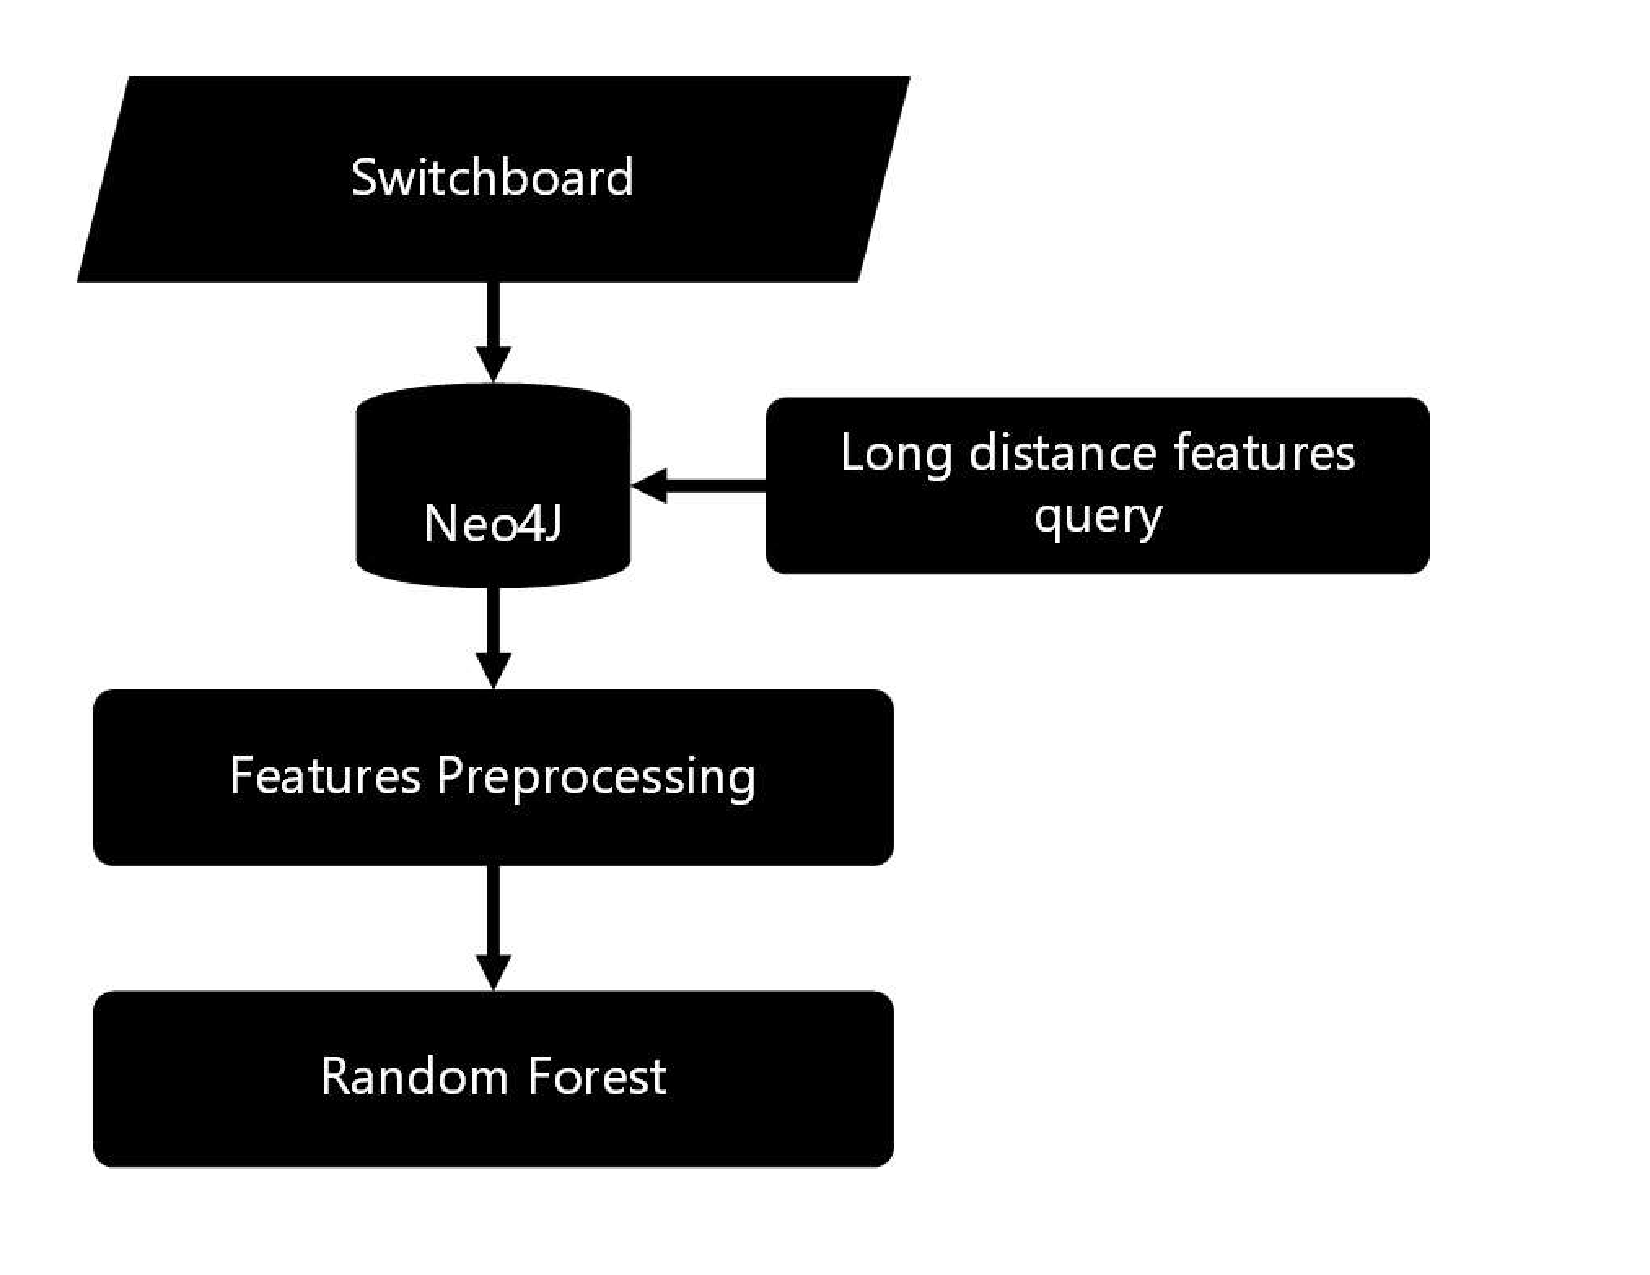
\includegraphics[width=10cm,keepaspectratio]{pipeline1.pdf}
 \caption{Experiment data pipeline
 \label{pipeline}}
 \end{figure}



\begin{figure}[ht!]
\centering
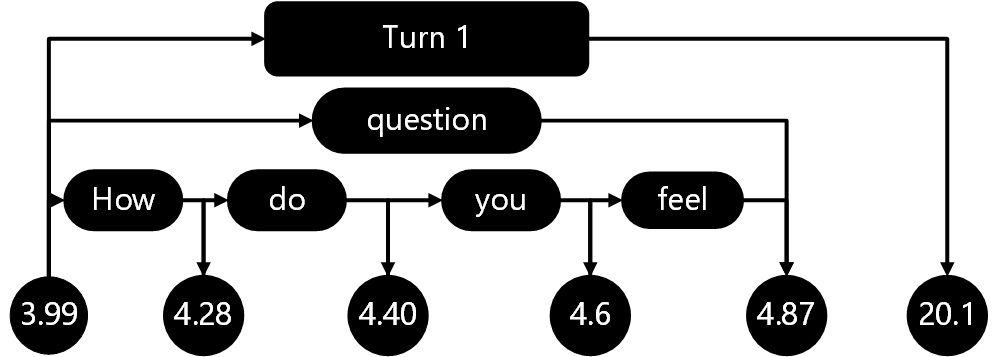
\includegraphics[width=10cm,keepaspectratio]{graph5.jpg}
\caption{Conversation graph data model \label{datastructure}}
\end{figure}

   After computing the summary features, we perform the following data transformation:
    \begin{itemize}[leftmargin=1em]
    \item We exclude 11 dialogue acts that were coded in Switchboard as ``other.''
    \item We filtered out all the dialogs that had data integrity issues,  for example
          dialog acts that referred to non existent terminals. This decrease the number
          of conversations from 624 to 310 conversations consisting of 60595 dialog acts.
    \item To reduce data sparsity, we grouped switchboard dialog acts into dialog act classes. This reduced the number of dialog acts from 148 to 9 dialog act classes. See Table 1 for examples of the mapping.
    \item We added a binary $y_{i+1}$ feature to each dialog act. As explained in Section 3, the variable is 1 if there is a turn change from dialogue act $d_i$ to $d_{i+1}$.

    \end{itemize}
    \begin{table}
     \begin{center}
    \begin{tabular}{ |p{2cm}||p{3cm} | }
    \hline
Switchboard dialog acts &  Dialog act classes  \\
    \hline
sd,h,bf      & statement   \\
sv,ad,sv@    & statement - opinion  \\
aa,aa\^r     & agree accept \\
\%.\%-,\%@   & abandon      \\
b,bh         & backchannel  \\
qy,qo,qh     & question     \\
no,ny,ng,arp & answer       \\
+            & +            \\
o@,+@        & NA           \\
  \hline
\end{tabular}
\end{center}\vspace{-0.5em}
\caption{Mapping from dialog act to dialog act class}
\label{tab:mapping}
\end{table}
